\documentclass[10pt,twocolumn]{article}
\usepackage[utf8]{inputenc}
\usepackage[T1]{fontenc}
\usepackage{lmodern}
\usepackage[a4paper,top=18mm,bottom=20mm,left=17mm,right=17mm,columnsep=7mm]{geometry}
\usepackage{microtype}
\usepackage{amsmath,amssymb,amsthm}
\usepackage{booktabs,tabularx,array}
\usepackage{enumitem}
\usepackage{graphicx,xcolor}
\usepackage{tikz}
\usetikzlibrary{arrows.meta,positioning,fit}
\usepackage{pgfplots}
\pgfplotsset{compat=1.18}
\usepackage{listings}
\usepackage{xurl,hyperref,cleveref,fancyhdr,titlesec}
\titleformat{\section}{\raggedright\normalfont\Large\bfseries}{\thesection}{1em}{}
\titleformat{\subsection}{\raggedright\normalfont\large\bfseries}{\thesubsection}{1em}{}
\hypersetup{hidelinks,pdftitle={PALO FinOps: Evidence-Gated Cost Accounting and Budget Admission for Multi-Model AI Workflows},pdfauthor={Fabrizio Degni},pdfsubject={AI FinOps, accounting provenance, budget admission and outcome measurement}}
\setlength{\parindent}{1em}
\setlength{\parskip}{0.1em}
\setlength{\headheight}{13pt}
\setlist{nosep,leftmargin=*}
\renewcommand{\arraystretch}{1.12}
\newcolumntype{Y}{>{\raggedright\arraybackslash}X}
\newcolumntype{P}[1]{>{\raggedright\arraybackslash}p{#1}}
\newtheorem{proposition}{Proposition}
\newcommand{\unavailable}{\mathsf{unavailable}}
\newcommand{\declared}{\mathsf{complete\_declared}}
\newcommand{\code}[1]{\texttt{#1}}
\pagestyle{fancy}
\fancyhf{}
\fancyhead[L]{\footnotesize PALO FinOps: accounting, authority and outcomes}
\fancyhead[R]{\footnotesize Degni, 2026}
\fancyfoot[C]{\thepage}
\renewcommand{\headrulewidth}{0.3pt}
\raggedbottom
\lstdefinestyle{palo}{basicstyle=\ttfamily\footnotesize,frame=single,breaklines=true,columns=fullflexible,keepspaces=true,showstringspaces=false,aboveskip=0.6em,belowskip=0.6em}

\begin{document}
\twocolumn[{%
\begin{@twocolumnfalse}
\begin{center}
\rule{\textwidth}{1.1pt}\\[0.65em]
{\fontsize{21}{24}\selectfont\bfseries PALO FinOps: Evidence-Gated\\Cost Accounting and Budget Admission\\for Multi-Model AI Workflows\par}
\vspace{0.8em}
{\large Fabrizio Degni\par}
\vspace{0.2em}
{\small PALO Framework - AI Ethics and Governance\\
\href{mailto:fabrizio.degni@gsom.polimi.it}{fabrizio.degni@gsom.polimi.it}\quad\url{https://paloframework.org}\par}
\vspace{0.5em}
{\small Technical preprint \quad Version 1.0 \quad 21 October 2026\par}
\end{center}
\begin{abstract}
The price of a model invocation is an incomplete basis for governing the cost of an AI workflow. Retries, unsuccessful attempts, context reconstruction, verification, shared infrastructure and human review can alter the cost per accepted outcome. At the same time, delayed billing and uncertain execution outcomes make a low observed total compatible with substantial unresolved liability. We present PALO FinOps, a reference model that separates four concerns: spending authority, operational commitments, versioned billing evidence and outcome-conditioned measurement. Its central rule is that incomplete evidence produces an unavailable final metric rather than an inferred zero cost. The model combines durable reservation before dispatch, explicit retention of unresolved commitments, revision-aware attribution, signed cost conservation and frozen metric contracts. A local implementation provides twelve operational capabilities, including role-oriented reporting, exception review, a read-only billing adapter, an isolated read-only Model Context Protocol server and a bounded routing benchmark runner. Evaluation comprises 63 local regression and integration tests, 20 focused interface checks and an exhaustive bounded enumeration of 12,864 signed-allocation configurations. Synthetic reconciliation examples demonstrate preservation of reservations, invalidation after billing revisions and replay of historical snapshots. These results establish executable behavior within the tested local scope; they do not establish provider billing accuracy, distributed enforcement, causal savings or production readiness. We conclude with a preregisterable live-evaluation protocol. The contribution is an explicit, testable contract connecting cost evidence to authority and outcomes, intended to complement routing algorithms and established FinOps practices.
\end{abstract}
{\small\noindent\textbf{Keywords:} AI FinOps; model routing; cost provenance; budget admission; financial accountability; outcome metrics; event journals; PALO.\par}
\vspace{0.7em}\rule{\textwidth}{0.5pt}\vspace{0.9em}
\end{@twocolumnfalse}
}]

\section{Introduction}

Multi-model AI workflows make resource consumption dependent on decisions taken during execution. A task may require several invocations, a model change, tool calls, verification and human correction. A failed attempt can consume resources without producing an accepted outcome. A timeout can leave both the execution result and the final charge unknown. Consequently, selecting a cheaper model and obtaining a cheaper accepted result are distinct propositions.

Prior work has established cost-aware model cascades and learned routing as useful optimization strategies~\cite{frugalgpt,routellm}. Agent evaluation research has also argued for joint consideration of cost, accuracy and reproducibility~\cite{agentsmatter}. Production-trace research identifies temporal dependencies in cache reuse across agentic turns and model changes~\cite{copilot}. These findings motivate measurement at the workflow level, but they do not by themselves determine when a particular organization's financial record is complete enough to support a decision.

Consider an operator observing a request that timed out after being sent. Counting it as free understates possible cost. Counting the entire reservation as an expense confuses capacity held for a possible charge with an incurred charge. Releasing the reservation and resubmitting may create a second paid attempt. Similarly, dividing a partly attributed bill by the number of successful tasks can produce a precise-looking number with incompatible scope. These are failures of accounting state and evidence interpretation, even when the routing algorithm behaves as designed.

PALO FinOps addresses this boundary through an explicit state model. It extends the PALO project's separation of proposed actions from externally granted authority~\cite{palo} to budget admission and financial evidence. The module is not an autonomous accountant: source finality, business acceptance and allocation drivers remain accountable declarations unless independently verified. Nor does it replace enterprise financial systems or claim compliance with a cost-data specification.

This paper makes three contributions:
\begin{enumerate}
\item A model separating operational commitments, billing attribution and accepted-outcome measurement, with conditional invariants and explicit unavailable states.
\item A reference implementation connecting these semantics to review workflows, local budget admission, a read-only evidence interface and a frozen routing experiment.
\item A reproducible synthetic evaluation and a proposed live protocol that distinguish accounting correctness from economic effectiveness.
\end{enumerate}

The research question is therefore bounded: \emph{can a local, explicit evidence contract prevent specified classes of accounting misstatement and unsafe resubmission in a multi-model workflow?} We evaluate this question through executable counterexamples and fault-oriented tests. Whether adopting the system improves organizational decisions or reduces real expenditure remains an empirical question.

\section{Related Work and Positioning}
\label{sec:related}

\subsection{Routing and agent evaluation}

FrugalGPT studies prompt adaptation, model approximation and cascades, including learned combinations of model calls~\cite{frugalgpt}. RouteLLM learns routing decisions from preference data to trade cost against response quality~\cite{routellm}. PALO FinOps does not introduce a competing routing estimator. A router can provide a candidate destination and a cost estimate, while the proposed accounting contract determines the applicable scope, reservation and evidence needed to interpret the outcome.

Kapoor et al. identify weaknesses in cost reporting, holdout design and reproducibility in agent benchmarks~\cite{agentsmatter}. Our emphasis on accepted outcomes and complete attempts is consistent with that work. We add an operational representation of incomplete billing and unresolved commitments; the general principle of evaluating cost alongside quality is not novel here.

Liu et al. characterize production coding-agent traces and report cache behavior that varies across turns and model switches~\cite{copilot}. This supports treating cache state and context reconstruction as experimental conditions. It does not imply that every switch is uneconomic, that another provider has the same cache behavior, or that cache invalidation translates one-for-one into billed expenditure. The present experiments do not reproduce their production dataset.

\subsection{FinOps and AI economics}

The FinOps Foundation's Unit Economics capability connects technology costs with business outcomes and asks practitioners to document metric definitions, sources and relationships~\cite{uniteconomics}. FOCUS provides a common vocabulary for cost and usage data; version 1.4 includes billed and effective costs, allocation information and correction handling~\cite{focus}. PALO preserves a declared cost basis and provenance rather than treating different bases as interchangeable. Its internal JSON format is not a FOCUS-conformant implementation.

LCOAI models lifecycle expenditure per productive AI output, including capital and operational components~\cite{lcoai}. Costa discusses fragmented governance, telemetry and FinOps in multi-provider AI adoption and develops outcome-oriented economic metrics~\cite{multilab}. These works are direct conceptual neighbors. Our narrower contribution is the executable handling of unknown cost, revision lineage, frozen cohorts and the separation of metric availability from dispatch authority. We make no first-system or first-metric claim.

Cloudability publicly describes allocation, business mapping, unit economics, anomaly management and forecasting~\cite{cloudability}. Such capabilities informed the operational requirements of the prototype. Our comparison is based on public product descriptions and demonstrations. It neither reconstructs a proprietary implementation nor tests feature parity, accuracy or performance against an authenticated commercial deployment. Vendor-reported savings are not used as experimental evidence for PALO.

\subsection{Transactions, identity and retries}

Atomic database transactions and request identities are established techniques. SQLite documents the assumptions under which a transaction survives interruption atomically~\cite{sqlite}. The Amazon Builders' Library discusses idempotency, retry ambiguity and reuse of request identifiers with different intent~\cite{retries}. PALO applies these ideas to the joint persistence of a request claim and a budget reservation. Its conservative local no-resend policy is not an end-to-end exactly-once execution guarantee.

\section{Scope, Entities and Assumptions}
\label{sec:model}

\subsection{Four distinct questions}

The model distinguishes: (i) \emph{may this principal initiate this request?}; (ii) \emph{how much local budget capacity is committed?}; (iii) \emph{what cost is supported by the selected billing evidence?}; and (iv) \emph{what cost can be assigned to a declared business outcome?} A positive answer to one question does not imply a positive answer to the others.

An implementation state is represented as
\begin{equation}
S=(W,J,L,A,O,M,P),
\end{equation}
where $W$ describes the workspace, workloads and budgets; $J$ is an operational event journal; $L$ is the versioned billing book; $A$ contains attribution links and allocation rules; $O$ contains declared task outcomes; $M$ contains metric contracts and frozen snapshots; and $P$ contains policy and principal scope. Currency is explicit, and no implicit foreign-exchange conversion is permitted.

A \emph{task} is a unit of intended work with an acceptance rule. An \emph{attempt} is one resource-consuming execution associated with that task. Several attempts can therefore contribute to one task, and unsuccessful attempts remain part of the numerator. An \emph{accepted outcome} is a task satisfying the declared rule, not simply an HTTP success or an LLM's assertion that it finished.

\subsection{Monetary representation and time}

Primitive monetary amounts are bounded integer micros, with $10^6$ micros per currency unit. Operational charges and reservations are nonnegative. Billing rows may be negative, for example when representing credits. Intermediate multiplication and division use integer or rational arithmetic where necessary to avoid silently losing precision. Derived unit ratios are not new charges: the new business-metric evaluator retains its numerator and denominator and provides an explicitly rounded display value.

Intervals are half-open UTC windows $[t_0,t_1)$. Usage and invoice periods are distinct concepts. The current importer declares usage coverage; it does not infer invoice-period completeness from that declaration. A source row crossing the selected boundary requires explicit periodization rather than an automatic proportional split.

\subsection{Trust and failure model}

The local runtime assumes that its host, configured credential boundary, SQLite database and validation code are trusted. It anticipates malformed imports, duplicated requests, conflicting identifiers, stale scopes, missing pages, delayed costs, concurrent reservations and process interruption. It does not defend against an administrator rewriting the database, a compromised host, a stolen provider credential or requests made outside the gateway.

Imported labels, evidence references and task outcomes are treated as data. A SHA-256 digest binds the content of a snapshot for replay; it does not authenticate an invoice issuer or prevent an attacker who controls both content and digest from replacing them. The term $\declared$ denotes consistency with the supplied declarations, not audited financial truth.

The configured gateway authenticates possession of a local secret and applies a workload and route allowlist. This is not enterprise OIDC or delegated end-user identity. The browser's role selector changes navigation only. A read-only evidence query cannot grant spending authority.

\section{Accounting and Admission Semantics}
\label{sec:semantics}

\subsection{Known cost and unresolved commitments}

Let $c_a$ be the known final operational charge for attempt $a$, or $\bot$ if unknown, and let $r_a$ be its reservation. For a scope $w$, define
\begin{align}
K_w &= \sum_{a\in w:\,c_a\ne\bot}c_a,\label{eq:known}\\
R_w &= \sum_{a\in w:\,c_a=\bot}r_a,\label{eq:reserved}\\
Q_w &= K_w+R_w.\label{eq:committed}
\end{align}
$K_w$ is known operational cost; $R_w$ is capacity held for unresolved attempts; $Q_w$ is committed capacity. Neither $R_w$ nor $Q_w$ is labeled final expenditure. A new reservation $r$ is admitted only if the configured identity, policy and request checks pass and
\begin{equation}
Q_w+r\le B_w\quad\land\quad Q_{\mathrm{all}}+r\le B_{\mathrm{all}},
\label{eq:admission}
\end{equation}
where $B_w$ and $B_{\mathrm{all}}$ are workload and workspace budgets. The reservation must also cover the declared estimate.

An unknown settlement retains $r_a$. A later reviewed reconciliation supplies a known $c_a$, removes that reservation from $R_w$ and includes $c_a$ in $K_w$. If $c_a>r_a$, the complete charge is retained and the overrun is reported. Thus \cref{eq:admission} is an admission predicate, not a theorem that final bills can never exceed budget.

\begin{proposition}[Local admission preservation]
Assume every reservation for a scope uses the same trusted journal and a serializable check-and-append transaction. Two concurrent requests cannot both be admitted on the basis of the same unconsumed local capacity.
\end{proposition}
\begin{proof}
The first committed transaction changes $R_w$. The next transaction evaluates \cref{eq:admission} against that changed state. If their combined reservations exceed either budget, the latter check fails. This argument does not cover a separate database, bypass path, external charge or erroneous estimate.
\end{proof}

\subsection{Request claims and dispatch}

The gateway binds a request identifier to its canonical content and configuration. The claim and reservation are inserted within one SQLite transaction. A failed insertion rolls back both. Only after commit may the process send the request to its fixed provider endpoint. Reuse of the identifier with the same binding returns the recorded state without another dispatch; a changed binding is rejected.

\begin{lstlisting}[style=palo,caption={Simplified local admission protocol. Network execution is outside the database transaction.},label={alg:dispatch}]
validate principal, scope, request
begin immediate transaction
  if request ID exists:
    require identical binding
    return recorded state
  require capacity and policy
  append reservation
  insert no-resend request claim
commit
send bounded provider request once
record receipt or uncertain state
retain reserve until reconciliation
\end{lstlisting}

\begin{proposition}[Conditional local no-resend]
For one request identifier in an intact persistent ledger, cooperating gateway instances following \cref{alg:dispatch} initiate at most one dispatch after successful claim creation.
\end{proposition}
\begin{proof}
Claim identity is unique and its check is serialized with insertion. Only the transaction creating the claim reaches the send path. Later instances observe the claim and return or reject. This does not establish that the remote provider executes exactly once; nor does it prevent a caller from expressing the same task under a new identifier.
\end{proof}

A crash after commit but before send can leave an unused reservation and an unresolved claim. This is an intentional safety-versus-liveness tradeoff: the prototype does not infer that nothing was sent and retry. Manual evidence-based recovery is required. Storage loss, rollback of the database or filesystem behavior outside SQLite's assumptions invalidates the argument~\cite{sqlite}.

\subsection{Billing revisions and conservation}

Each source row has an economic identity and a revision. Repeating the same content is idempotent; correction uses a higher revision with explicit lineage. Superseded rows remain historical evidence, while only active revisions enter a current projection. Links to an obsolete revision do not silently transfer to the replacement. Quarantined or incomplete imports remain visible and block completeness claims.

For a signed source amount $b_j$, define attributed shares $x_{jw}$ and a signed residual $u_j$:
\begin{equation}
b_j=\sum_w x_{jw}+u_j.
\label{eq:conservation}
\end{equation}
Shared allocations use integer weights and a largest-remainder allocation of the absolute amount, with a deterministic identifier tie-break, followed by restoration of the sign. A zero total weight leaves the full amount unallocated. Missing or expired rules therefore preserve the cost as a residual.

\begin{proposition}[Allocation conservation]
For a valid signed integer amount and valid nonnegative integer weights, the allocation procedure satisfies \cref{eq:conservation} exactly.
\end{proposition}
\begin{proof}
For positive total weight, floor division assigns an integer part of each proportional share. The difference between the absolute amount and the sum of these parts is distributed as individual micros according to the remainder order. Restoring the sign preserves the equality. If total weight is zero, every share is absent and $u_j=b_j$.
\end{proof}

Direct attempt links and shared allocation are separate attribution paths. They are not additional expenses to be added to their source rows. Likewise, operational ledger totals and the billing book describe overlapping financial activity and must not be summed as independent costs. The equality proves arithmetic conservation; it does not prove that the chosen driver is economically appropriate.

\subsection{Evidence-gated outcome metrics}

A metric contract fixes currency, accounting basis, interval, workload population, outcome rule, source and version. A frozen snapshot includes the exact book, operational state, rules and outcomes needed for replay. Let $C_\Gamma$ be attributed billing cost for cohort $\Gamma$, including attempts that did not succeed and allocated shared costs. Let $N_\Gamma$ count accepted attempted tasks in that cohort. Define
\begin{equation}
U_\Gamma=
\begin{cases}
C_\Gamma/N_\Gamma,&\chi(\Gamma)=1,\ N_\Gamma>0,\\
\unavailable,&\text{otherwise},
\end{cases}
\label{eq:metric}
\end{equation}
where $\chi$ is a conjunction of completeness predicates: closed time window, complete declared import coverage, compatible scope and basis, no unresolved quarantine, final source revisions, resolved attribution, agreement between linked bills and operational charges, and no pending outcomes. The implementation conservatively checks the relevant billing partition; uncertainty elsewhere in that partition can also block a selected-workload metric.

General business metrics replace $N_\Gamma$ with an observed, versioned denominator bound to the same cohort digest. The current implementation retains the accepted-task snapshot's completeness gates. It may therefore reject a metric that a more permissive domain-specific model could calculate. Forecast denominators are never mixed into observed results. Corrections create new versions or snapshots; they do not rewrite a prior result.

The protocol withholds a final ratio, not all information. A provisional report can still display known costs, outstanding reservations, source totals, attributed amounts and reasons for unavailability. This makes missing evidence an operational object rather than an invisible assumption.

\section{Reference Architecture and Workflows}
\label{sec:architecture}

\begin{figure*}[t]
\centering
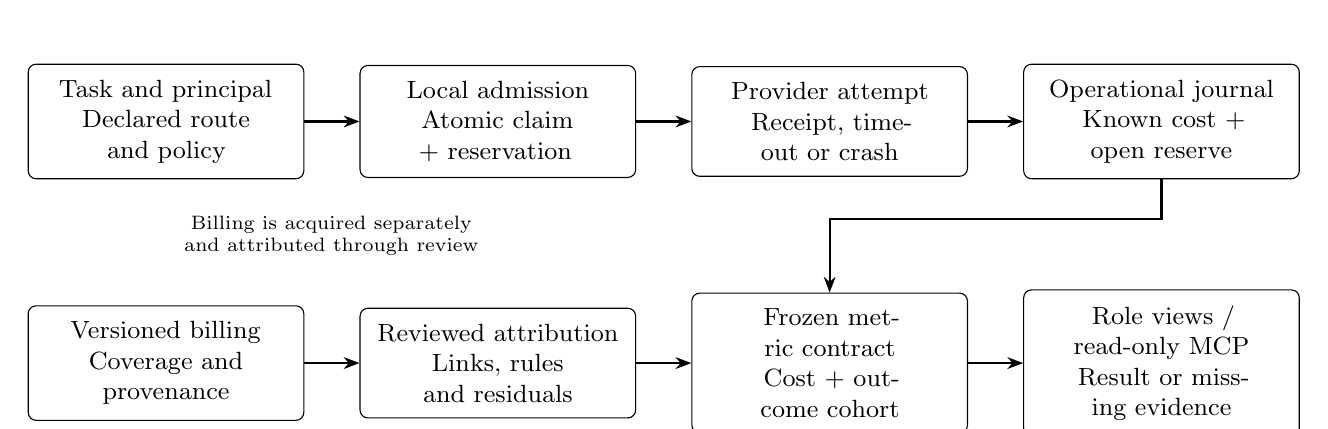
\begin{tikzpicture}[font=\small,box/.style={draw,rounded corners=1mm,align=center,minimum height=13mm,text width=31mm,inner sep=2mm},arr/.style={-{Stealth[length=2mm]},thick},node distance=7mm and 7mm]
\node[box] (request) {Task and principal\\Declared route and policy};
\node[box,right=of request] (gateway) {Local admission\\Atomic claim + reservation};
\node[box,right=of gateway] (provider) {Provider attempt\\Receipt, timeout or crash};
\node[box,right=of provider] (journal) {Operational journal\\Known cost + open reserve};
\node[box,below=16mm of request] (billing) {Versioned billing\\Coverage and provenance};
\node[box,right=of billing] (allocation) {Reviewed attribution\\Links, rules and residuals};
\node[box,right=of allocation] (snapshot) {Frozen metric contract\\Cost + outcome cohort};
\node[box,right=of snapshot] (reports) {Role views / read-only MCP\\Result or missing evidence};
\draw[arr] (request)--(gateway);
\draw[arr] (gateway)--(provider);
\draw[arr] (provider)--(journal);
\draw[arr] (billing)--(allocation);
\draw[arr] (allocation)--(snapshot);
\draw[arr] (snapshot)--(reports);
\draw[arr] (journal.south)--++(0,-5mm)-|(snapshot.north);
\node[font=\scriptsize,align=center] at (2.1,-1.45) {Billing is acquired separately\\and attributed through review};
\end{tikzpicture}
\caption{Separation of spending authority and financial evidence. The upper flow controls local admission and records operational state; the lower flow acquires and interprets billing. A receipt does not automatically establish a final cost. Read-only analysis has no reverse path that authorizes execution. The diagram describes the reference architecture, not an authenticated production deployment.}
\label{fig:architecture}
\end{figure*}

\subsection{Browser workspace and review}

The implementation has a browser workspace and a separate Node.js runtime (\cref{fig:architecture}). The browser contains no provider credential and makes no model execution request. It exposes twelve capabilities summarized in \cref{tab:capabilities}. CFO, IT lead, administrator and AI service owner entry points share the same data but emphasize different decisions.

Exceptions cover unresolved costs, missing imports, quarantined data, residuals, missing drivers, estimated sources and pending outcomes. Stable case identities prevent repeated observations from becoming independent incidents. Reviews retain owner, reason and history; new source evidence can reopen the case. Closing a case is administrative and cannot settle a cost or release a reservation. This prevents a workflow status from being mistaken for an accounting event.

A CFO report separates whole-workspace budget commitments from selected-period attributed billing. It states period, currency, basis and completeness. A filtered export is labeled as a selection, while a complete workspace export preserves the book, rules and optional operations state. No complete-declared report is presented as an independently audited invoice or a statutory financial statement.

An opportunity moves through proposed, approved, applied and measured states. A measured comparison requires verified snapshots for non-overlapping periods, a declared comparability review, quality constraints and intervention cost. For baseline $(C_0,N_0)$ and follow-up $(C_1,N_1)$, the observed normalized difference is
\begin{equation}
D=\frac{C_0N_1}{N_0}-C_1-C_{\mathrm{intervention}}.
\label{eq:difference}
\end{equation}
The implementation retains the exact normalization terms and rounds the difference once for display. A positive $D$ is not labeled a causal saving. Changes in workload composition, prices, credits or acceptance practices can explain it. Rule-comparison previews similarly show allocation sensitivity without changing the book or declaring operational savings.

\subsection{Billing adapter and bounded gateway}

The initial adapter reads OpenAI organization Costs data from a fixed endpoint with explicit organization, project, currency and interval checks~\cite{openaicosts}. It requires complete daily coverage, bounded pagination and valid cursor behavior. A missing bucket is not invented as a zero day; an explicit empty bucket is accepted. Whether every selected real account supplies such zero buckets remains a pilot compatibility question.

The adapter produces estimated shared rows because daily project and line-item aggregates do not independently establish per-attempt attribution or final invoice status. Finalization requires authoritative external evidence and an explicit revision. It must not be achieved simply by relabeling an estimate to make a metric available.

The gateway accepts bounded text requests and uses a fixed Responses endpoint~\cite{openairesponses}. It checks principal, policy digest, workload, route, time bounds and reservation before dispatch. The estimate uses input bytes, a declared framing allowance and versioned rates. This is a reviewed estimation procedure, not a proof of a provider-enforced dollar ceiling. There is no automatic retry, arbitrary destination URL or model-selected tool invocation. Receipts include identifiers, route, rate version, policy digest, elapsed time and usage; raw prompt text is not included in them. Returned model output remains task data requiring appropriate protection.

Successful usage telemetry leaves the final cost unknown until reconciliation. The prototype also has no universal automatic adjustment path for already settled attempts when a later invoice revision changes their cost. Such a revision can invalidate the current metric and require explicit accounting repair; preserving the discrepancy is preferable to silently changing a settled history.

\subsection{Read-only evidence access}

An isolated stdio Model Context Protocol server exposes four tools: summary, exceptions, cost explanation and period snapshot. The host binds an exact workspace and a frozen finance bundle at startup. Authentication precedes access; expiry is rechecked during queries. The model cannot supply a path, select another tenant or invoke a settlement, budget change or execution tool.

Responses cite the workspace and bundle digest, and period results cite their frozen scope and snapshot. These references improve inspectability but are not signatures or proof of source authenticity. The current identity boundary is local process access plus a secret; a network transport would require its own authentication and isolation design.

\subsection{Forecasting as a separate analytical view}

The forecast capability uses consecutive complete daily observations ending on the last closed UTC day. It compares last-value and trailing-seven-observation mean baselines with rolling one-step origins. The holdout is used for selection, so the selected score is not an independent final generalization estimate. Multi-day output holds the selected final estimate constant; it has no calibrated uncertainty interval.

Gaps, insufficient history and open-day observations block output. Net-negative days are rejected by this pilot rather than clipped; credit treatment requires an explicitly defined upstream series. A forecast never changes $B_w$ or creates permission to spend. This deliberately modest baseline avoids interpreting a sophisticated-looking projection as authority.

\section{Routing Economics and Experimental Contract}
\label{sec:routing}

\subsection{Remaining cost, not model price alone}

At a proposed switch, both alternatives must use the same remaining task horizon. For strategy $s$, write
\begin{equation}
\widehat C_s=\widehat C_{s,\mathrm{model}}+
\widehat C_{s,\mathrm{tools}}+
\widehat C_{s,\mathrm{review}}+
\widehat C_{s,\mathrm{other}}.
\label{eq:fullcost}
\end{equation}
These categories must be disjoint. Context replay and cache reconstruction may already be charged as model input; they must not be added again as a separate fee. Likewise, provider counters that include cached tokens within total input require a mapping that avoids overlapping token categories. Latency is reported separately unless an explicit business rule monetizes it.

The reference transition assessment uses a declared uncertainty margin $m$ and an economic condition
\begin{equation}
\widehat C_{\mathrm{stay}}-\widehat C_{\mathrm{switch}}>m.
\end{equation}
It also checks destination identity, current rates, policy, disclosure references, quality evidence, unresolved effects and budget coverage. Passing the assessment alone neither authorizes execution nor demonstrates that the estimates are calibrated. Unknown cache state may be compatible with an explicit worst-case reservation, but the prototype does not prove that a supplied bound is conservative. Excluding a common sunk cost from both alternatives is valid; including it on only one side is not.

\subsection{Frozen paired execution}

The prepared benchmark runs two stages per task. The stay strategy uses model A twice; the switch strategy uses A then B. The same first-stage route and rate version are required. Prompts, follow-up template, expected final answer, cache-condition declaration, routes and reservations are frozen before execution. Strategy order alternates across tasks; this mitigates a simple order effect but does not isolate cache state, load or temporal drift.

Every attempted stage remains recorded, including failed or interrupted stages. The current runner has no automatic retries. Additional retries in an expanded experiment must become additional attributable attempts, not replace failures in the record. Acceptance is exact match after trimming, which suits narrow deterministic tasks but not open-ended quality evaluation.

The analyzer requires final measured attribution, no relevant unresolved liabilities or source residuals, and an ancillary-cost declaration for each task and strategy. An explicit zero is a declaration requiring evidence; absence is not zero. It verifies bindings among plan, attempts, route versions and receipts. It withholds final cost per accepted outcome when the contract is incomplete. A complete declared comparison still does not establish causal savings or general superiority of one model family.

\section{Evaluation}
\label{sec:evaluation}

\subsection{Method and evidence scope}

We distinguish three evaluations. First, the implementation's local test suite exercises accounting and runtime behavior. Second, bounded deterministic enumeration probes the signed allocation function. Third, a synthetic reconciliation sequence and an arithmetic sensitivity example expose interpretation errors. All use synthetic inputs; no paid provider execution or authenticated invoice capture is part of these results. Fixture timestamps use a simulated clock, including a closed billing period, and are not observations of future activity.

The implementation snapshot was checked on 21 October 2026. Its test receipt contains 63 passing tests, no failures and no skipped tests. Coverage includes duplicate and overlapping imports, explicit revisions, credits, allocation, metric replay, scope and authentication denial, concurrent budget writers, gateway request duplication, rollback on claim insertion failure and process termination during dispatch. The MCP test initializes the actual local JSON-RPC stdio server, enumerates the four tools and exercises permitted and rejected requests. Provider transports in these tests are injected synthetic responses.

Twenty additional interface-harness checks passed. They cover selected state and navigation behaviors, replacement handling, labeling and identifiers; they use a minimal DOM and are not a usability study. Separate browser observations exercised the nine Operations panels and narrow-viewport geometry. These UI checks support interaction consistency, not financial or security validity. Test counts are not estimates of production reliability or coverage percentages.

\subsection{Bounded allocation enumeration}

The paper's companion script calls the implementation for every integer amount in $[-100,100]$ micros and every three-destination weight vector in $\{0,1,2,3\}^3$. This yields
\begin{equation}
201\times4^3=12{,}864
\end{equation}
configurations. Each checks conservation including the residual, invariance under reversal of input destination order, and safe-integer output shares. All 38,592 assertions passed. For example, a credit of $-7$ micros with equal weights is assigned as $(-3,-2,-2)$ in identifier order.

This enumeration is exhaustive only over the stated small domain. It is not a random sample, an independent statistical trial set, or proof that every surrounding import and allocation policy is correct. The algebraic conservation argument is conditional on valid inputs; the enumeration checks agreement of selected implementation behavior with that argument.

\subsection{Synthetic accounting sequence}

\Cref{tab:sequence} reports values produced by the implementation, not hand-entered benchmark outcomes. The initial example has four attempts, known operational cost of USD~0.34 and an unresolved reservation of USD~0.18. With a budget of USD~1.50, remaining capacity is USD~0.98. The period metric is unavailable because an attempt cost and a task outcome remain unresolved.

\begin{table}[t]
\centering\small
\begin{tabularx}{\columnwidth}{@{}Yrr@{}}
\toprule
State or operation & Value (USD) & Final metric\\
\midrule
Initial known cost & 0.3400 & unavailable\\
Initial open reserve & 0.1800 & unavailable\\
Case closed administratively & 0.1800$^{a}$ & unavailable\\
Reviewed operational total & 0.4400 & separate view\\
Attributed billing total & 0.4670 & complete$^{b}$\\
Cost per accepted task & 0.2335 & complete$^{b}$\\
Repeated import total & 0.4670 & unchanged\\
Revised source total & 0.4870 & unavailable\\
\bottomrule
\end{tabularx}
\caption{Synthetic accounting sequence. $^{a}$Open reserve remains unchanged. $^{b}$Complete under declarations only, with two accepted tasks; provider verification remains false. The operational total and billing total must not be added.}
\label{tab:sequence}
\end{table}

Closing the exception preserves the reservation. Reviewed reconciliation then assigns USD~0.10 to the unresolved attempt and marks its task failed, yielding USD~0.44 of known operational cost and no open reservation. The billing book also contains a USD~0.03 shared pool and a USD~$-0.003$ shared credit. Total attributed billing is therefore USD~0.467, and dividing by two accepted tasks gives USD~0.2335. Failed work remains represented in the numerator.

Repeating the import leaves the total at USD~0.467. Revising one source row from USD~0.22 to USD~0.24 yields USD~0.487 of current source cost, but invalidates its old attribution and makes the new metric unavailable. The previous frozen snapshot still verifies and retains its original result. This behavior demonstrates preservation of historical evidence alongside current incompleteness, not automatic repair of financial truth.

A separate business denominator of three units gives the exact ratio $467{,}000/3$ micros. The displayed value is 155,667 micros under nearest-micro rounding with ties away from zero; the original ratio is retained. A mismatched cohort digest blocks evaluation. Expiring the shared-cost rules leaves the pool and credit unallocated and also blocks the period metric.

\subsection{Constructed routing counterexample}

\begin{figure}[t]
\centering
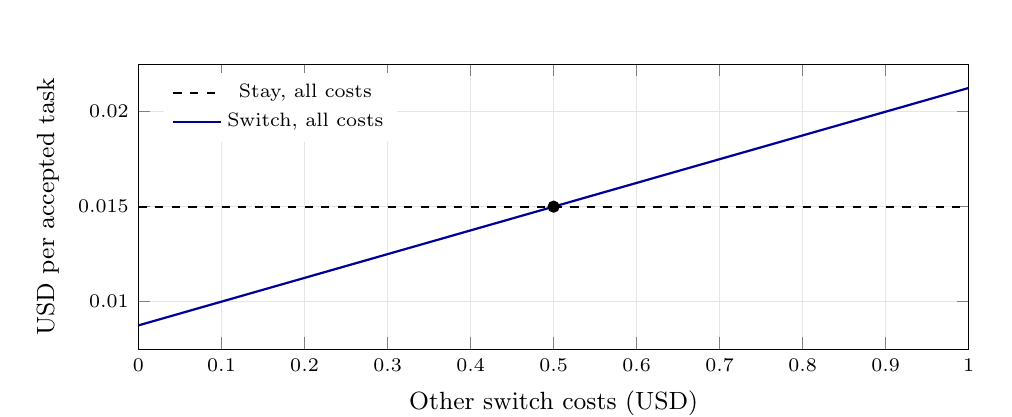
\begin{tikzpicture}
\begin{axis}[width=\columnwidth,height=52mm,xmin=0,xmax=1,ymin=0.0075,ymax=0.0225,xlabel={Other switch costs (USD)},ylabel={USD per accepted task},tick label style={font=\scriptsize},label style={font=\small},legend style={font=\scriptsize,at={(0.03,0.97)},anchor=north west,draw=none,fill=white},scaled y ticks=false,ytick={0.01,0.015,0.02},yticklabel style={/pgf/number format/fixed,/pgf/number format/precision=3},grid=major,grid style={gray!20}]
\addplot[black,thick,dashed] coordinates {(0,0.015) (1,0.015)};
\addlegendentry{Stay, all costs}
\addplot[blue!60!black,thick] coordinates {(0.0000,0.00875000) (0.0125,0.00890625) (0.0250,0.00906250) (0.0375,0.00921875) (0.0500,0.00937500) (0.0625,0.00953125) (0.0750,0.00968750) (0.0875,0.00984375) (0.1000,0.01000000) (0.1125,0.01015625) (0.1250,0.01031250) (0.1375,0.01046875) (0.1500,0.01062500) (0.1625,0.01078125) (0.1750,0.01093750) (0.1875,0.01109375) (0.2000,0.01125000) (0.2125,0.01140625) (0.2250,0.01156250) (0.2375,0.01171875) (0.2500,0.01187500) (0.2625,0.01203125) (0.2750,0.01218750) (0.2875,0.01234375) (0.3000,0.01250000) (0.3125,0.01265625) (0.3250,0.01281250) (0.3375,0.01296875) (0.3500,0.01312500) (0.3625,0.01328125) (0.3750,0.01343750) (0.3875,0.01359375) (0.4000,0.01375000) (0.4125,0.01390625) (0.4250,0.01406250) (0.4375,0.01421875) (0.4500,0.01437500) (0.4625,0.01453125) (0.4750,0.01468750) (0.4875,0.01484375) (0.5000,0.01500000) (0.5125,0.01515625) (0.5250,0.01531250) (0.5375,0.01546875) (0.5500,0.01562500) (0.5625,0.01578125) (0.5750,0.01593750) (0.5875,0.01609375) (0.6000,0.01625000) (0.6125,0.01640625) (0.6250,0.01656250) (0.6375,0.01671875) (0.6500,0.01687500) (0.6625,0.01703125) (0.6750,0.01718750) (0.6875,0.01734375) (0.7000,0.01750000) (0.7125,0.01765625) (0.7250,0.01781250) (0.7375,0.01796875) (0.7500,0.01812500) (0.7625,0.01828125) (0.7750,0.01843750) (0.7875,0.01859375) (0.8000,0.01875000) (0.8125,0.01890625) (0.8250,0.01906250) (0.8375,0.01921875) (0.8500,0.01937500) (0.8625,0.01953125) (0.8750,0.01968750) (0.8875,0.01984375) (0.9000,0.02000000) (0.9125,0.02015625) (0.9250,0.02031250) (0.9375,0.02046875) (0.9500,0.02062500) (0.9625,0.02078125) (0.9750,0.02093750) (0.9875,0.02109375) (1.0000,0.02125000)};
\addlegendentry{Switch, all costs}
\addplot[only marks,mark=*,black] coordinates {(0.5,0.015)};
\end{axis}
\end{tikzpicture}

\caption{Constructed arithmetic sensitivity, not measured model performance. Both strategies have 80 declared accepted tasks out of 100. Stay costs USD~1.00 in inference plus USD~0.20 elsewhere; switch costs USD~0.70 in inference plus the horizontal-axis amount. Other costs are non-overlapping with the inference total. The crossover is USD~0.50.}
\label{fig:sensitivity}
\end{figure}

\Cref{fig:sensitivity} holds acceptance fixed to isolate accounting scope. On an inference-only comparison, USD~0.70 appears cheaper than USD~1.00. Including USD~0.20 of other costs for stay yields USD~0.015 per accepted task. Switch breaks even when its other costs reach USD~0.50. At USD~0.60, switch costs USD~0.01625 per accepted task despite its lower inference bill.

These numbers are intentionally constructed. They establish that the ranking can reverse under a broader cost definition; they do not estimate how often it reverses in practice. The companion script generates 81 points on this arithmetic curve. No sampling error, confidence interval or provider-price inference is attached to it.

\subsection{Fault-oriented review}

An actual GLM-5.3 review of selected implementation files identified a crash window in the first claim/reservation design and imprecise treatment of fractional unit values. The implementation was revised to commit claim and reservation atomically and to retain exact rational terms for the new calculations. Regression tests cover rollback after an injected claim-insertion error and non-integral thirds. Other model-generated concerns were checked against the omitted billing code rather than accepted on authority.

This review was a development aid, not a second empirical evaluator. GLM did not run the tests, inspect a real account or approve the corrected manuscript. Its initial review and the subsequent adjudication are preserved in the local implementation evidence. The present paper relies on source inspection, executable receipts and the stated assumptions, not on a model's endorsement.

\section{Limitations and Threats to Validity}
\label{sec:limits}

\paragraph{Construct validity.}
An accepted task is only as meaningful as its acceptance rule and outcome source. Exact match is inadequate for many business tasks. A favorable cost-per-outcome ratio can conceal unequal difficulty, different error severity or lower coverage. Normalizing by volume does not correct those differences. A metric contract makes assumptions inspectable but does not establish their business validity.

\paragraph{Source validity.}
Complete-declared coverage, finality labels and review references can be wrong. Aggregate API costs do not independently establish final invoice amounts or attempt-level attribution. Credits can reduce net cost without reflecting operational improvement. The conservative treatment of missing daily buckets may reject usable provider extracts; relaxing it would require evidence of the provider's zero-reporting convention. Invoice periods and usage windows remain distinct.

\paragraph{Internal validity.}
Implementation tests and the paper's fixtures share code and design assumptions, so correlated errors are possible. Small-domain enumeration is not a verification of all numerical boundaries, all event sequences or economic policies. The conditional propositions are mathematical arguments about simplified procedures, not machine-checked proofs of the JavaScript implementation. UI checks do not establish accessibility, human comprehension or error rates in use.

\paragraph{External validity.}
No production deployment, paid routing experiment, live provider reconciliation or enterprise identity integration has been validated. The pilot uses a single configured account scope and one currency. It does not evaluate multi-region database replication, distributed leases, chargebacks, amortization policy, tax, exchange-rate treatment or cross-provider invoice reconciliation. No commercial system was tested head-to-head.

\paragraph{Safety and liveness.}
The no-resend rule deliberately holds uncertain requests, including some that never reached the provider. This can reduce availability and require costly human review. New identifiers can circumvent semantic deduplication unless a higher-level workflow binds them. The database and host are trusted; integrity against a privileged adversary is outside the prototype. The gateway's estimate is not a provider-enforced spend cap, and settled overruns remain possible.

\paragraph{Economic effectiveness.}
Logging, reconciliation, verification and review themselves cost money and time. They must be included when evaluating adoption. The current record demonstrates neither net savings nor better decisions. Withholding a metric avoids false precision but can also delay useful action; an empirical study should measure that tradeoff. The intentionally conservative business-metric gates and missing-bucket policy may need domain-specific refinements.

\paragraph{Privacy and evidence minimization.}
Receipts avoid raw prompts, but configuration, workload identifiers, model outputs and business denominators may still reveal sensitive activity. A digest is not anonymization; low-entropy data can be guessed. The browser's local storage is not a multi-user authorization boundary. Production evidence retention requires an explicit access, minimization and deletion policy beyond the local prototype.

\section{Proposed Live Validation Protocol}
\label{sec:future}

The next study should be preregistered before paid execution. It should freeze the provider account, model and rate versions, task population, acceptance rubric, workload scope, exclusion rules and accounting basis. A real extract should first be reconciled against the read-only adapter, including empty days, credits, corrections and late records. The goal is to characterize discrepancies and coverage, not to assume that a successful API call proves completeness.

For routing, a paired task design should compare a competent stay baseline with the declared switch strategy. Tasks should be stratified by relevant complexity. Repeated trials, randomized or counterbalanced order, provider cache conditions and temporal load should be documented. The implementation's alternating-order runner is a starting point; it does not yet supply this full design. Exact-match tasks may be used initially, followed by a separately validated rubric and blinded human assessment for open-ended tasks.

Primary outcomes should include attributed total cost per accepted task, acceptance rate, unresolved-cost rate and time to reconciliation. Secondary outcomes should include latency, review effort, provider/API discrepancies, admission denials, retained uncertain reservations and duplicate dispatch attempts. All failures and ancillary review costs must remain in scope. A follow-up study should measure the rate at which the system correctly withholds a metric and the operational cost of unnecessary withholding.

Sample size should be chosen from pilot variance and a declared minimum relevant difference, not inferred from the number of software tests. Confidence intervals should respect task-level pairing and dependence among attempts. Quality non-inferiority should be specified before comparing costs. No superiority claim should be made while unmatched liabilities, unassigned costs or unresolved quality differences remain. Independent replication should use the frozen source manifest and its own provider evidence.

\section{Conclusion}

PALO FinOps connects budget admission to an explicit accounting and outcome-evidence model. Its practical rule is that missing information remains missing: an uncertain attempt retains its reservation, a revised bill can invalidate current attribution, and an incomplete cohort does not produce a final unit cost. These rules complement model routing and established FinOps practices by making the evidence boundary executable.

The reference implementation and synthetic evaluation show that the specified behaviors can be exercised consistently within a local trusted runtime. They do not show that routing becomes cheaper, that invoices are independently verified, or that the architecture is production-ready. The next contribution must come from live reconciliation, controlled comparative execution and independent assessment of both economic benefits and review costs.

\section*{Competing Interests}
The author conceived and maintains PALO Framework and has an intellectual and reputational interest in the model. Public product documentation informed requirements; no endorsement by the cited researchers, vendors or foundations is implied.

\section*{AI Assistance and Author Responsibility}
Codex assisted with implementation, literature retrieval, drafting, reproducibility scripts and document preparation. GLM-5.3 supplied the implementation critique described in \cref{sec:evaluation}; it did not validate the reported experiments or review this manuscript. AI tools are not authors or independent validators. The author remains responsible for reviewing the full content, source attributions and any subsequent scholarly submission.

\section*{Data and Artifact Availability}
The general PALO project is available at \url{https://github.com/sev7enITA/PALOframework}. This paper concerns the FinOps 1.2 reference implementation. The companion release is identified by its source commit and artifact hashes; the module and download links are provided at \url{https://paloframework.org/PALO_FinOps.html}. The companion package contains the synthetic experiment script, input fixtures, relevant source modules, results and source hashes. The local implementation evidence separately preserves the 63-test receipt and review records. A permanent public identifier for this exact artifact has not yet been assigned. No confidential customer data or live billing records were used.

\appendix
\section{Capability and Evidence Map}
\label{sec:capabilities}

\begin{table*}[t]
\centering\small
\begin{tabularx}{\textwidth}{@{}P{7mm}P{35mm}YP{43mm}@{}}
\toprule
ID & Capability & Implemented behavior & Present evidence boundary\\
\midrule
1 & Role entry views & CFO, IT, administrator and service owner navigation over shared data. & Local UI; role selection is not access control.\\
2 & Exception queue & Deduplication, source-sensitive reopening and review history. & Closing a case cannot change accounting.\\
3 & Cost explanation & Source revision, driver, rule, shares, residuals and attempt links. & Arithmetic provenance; driver validity remains declared.\\
4 & Business metrics & Versioned contract and observed denominator bound to a frozen cohort. & Incomplete or mismatched inputs withhold a ratio.\\
5 & Opportunity lifecycle & Proposed, approved, applied and measured stages with evidence. & Observed comparison; no causal-savings claim.\\
6 & CFO period package & Frozen scope, completeness, selected export and full archive. & Declared completeness; not an audited financial statement.\\
7 & Allocation preview & Frozen before/after rule projections with signed deltas. & Sensitivity; no automatic rule application or savings.\\
8 & Read-only connector & Fixed Costs API, explicit scope, coverage and revision mapping. & Synthetic transport tested; real extract pending.\\
9 & Forecast & Chronological baseline comparison on complete daily data. & Selection score is not an independent final test.\\
10 & Read-only MCP & Four scoped tools on a host-bound frozen bundle. & Actual local protocol tested; local-secret identity.\\
11 & Routing benchmark & Frozen two-stage stay/switch plan and complete-cost checks. & Synthetic execution; paid trials and final bills pending.\\
12 & Controlled gateway & Atomic claim/reservation, scoped dispatch and receipts. & Local fault tests; real receipts and production qualification pending.\\
\bottomrule
\end{tabularx}
\caption{Twelve implemented capabilities and the limits of their current validation. A code path is not evidence that its live operational pilot has been completed.}
\label{tab:capabilities}
\end{table*}

\Cref{tab:capabilities} maps the research requirements to implementation behavior. The local browser adds nine Operations panels while retaining the existing overview, ledger, reconciliation, billing, route assessment and setup surfaces. The runtime components are separate from the browser and from the older loopback-only probe.

\section{Reproduction and Falsification}
\label{sec:repro}

The pure synthetic experiment uses Node.js v22.22.3 in the recorded run and makes no network requests. From the companion package root:
\begin{lstlisting}[style=palo]
node papers/palo-finops-arxiv/reproducibility/experiments.mjs
\end{lstlisting}
It writes the numerical results and hashes of the source modules and fixtures. The broader implementation suite requires the repository's locked dependencies and a Node runtime with the SQLite functionality used by the pilot:
\begin{lstlisting}[style=palo]
npm run finops:check
\end{lstlisting}
Its 63-test result is a dated receipt for the evaluated source snapshot. It should not be assumed to apply unchanged to a later checkout. The pure companion package reproduces the allocation enumeration and accounting examples; it is not a standalone distribution of every UI and runtime integration test.

Examples of falsifying observations are: conservation failure for valid inputs; a repeated identical import changing current cost; a case closure releasing a reservation; a mismatched cohort producing a final ratio; an unchanged request identifier causing a second local dispatch; or an incomplete source becoming complete without new evidence. A live provider bill above the reservation would falsify a claimed hard cap, which is why no such cap is claimed. A negative net economic result would not contradict arithmetic correctness but would undermine the business case for adoption.

\section{Interpretation of Result Labels}

\noindent\textbf{Known operational cost:} a charge recorded in the operational journal; its provenance remains explicit.\\
\textbf{Open reservation:} local capacity held for an unresolved attempt, not final expenditure.\\
\textbf{Estimated billing:} imported cost that has not met the declared finality requirement.\\
\textbf{Complete declared:} the supplied accounting, scope and outcome predicates agree; provider authenticity and independent audit are not implied.\\
\textbf{Unavailable:} one or more required predicates are missing or inconsistent; diagnostic values may still be displayed.\\
\textbf{Observed difference:} a comparison of declared periods with explicit normalization and quality constraints; causal savings are not inferred.\\
\textbf{Admitted:} local identity, policy and capacity checks passed; remote execution and final cost remain separate facts.

\begin{thebibliography}{99}
\small
\raggedright
\setlength{\itemsep}{3pt}
\bibitem{frugalgpt}
L. Chen, M. Zaharia and J. Zou. FrugalGPT: How to Use Large Language Models While Reducing Cost and Improving Performance. \href{https://arxiv.org/abs/2305.05176}{arXiv:2305.05176}, 2023.

\bibitem{routellm}
I. Ong, A. Almahairi, V. Wu, W.-L. Chiang, T. Wu, J. E. Gonzalez, M. W. Kadous and I. Stoica. RouteLLM: Learning to Route LLMs with Preference Data. \href{https://arxiv.org/abs/2406.18665v4}{arXiv:2406.18665v4}, 2025; first submitted 2024.

\bibitem{agentsmatter}
S. Kapoor, B. Stroebl, Z. S. Siegel, N. Nadgir and A. Narayanan. AI Agents That Matter. \href{https://arxiv.org/abs/2407.01502}{arXiv:2407.01502}, 2024.

\bibitem{copilot}
B. Liu, H. Qiu, \mbox{\'I\~nigo Goiri}, R. Fonseca, R. Bianchini and E. Choukse. Agentic Coding in the Wild: Characterizing GitHub Copilot Traces at Production Scale. \href{https://arxiv.org/abs/2608.00101}{arXiv:2608.00101}, 2026.

\bibitem{uniteconomics}
FinOps Foundation. \href{https://www.finops.org/framework/capabilities/unit-economics/}{Unit Economics}. FinOps Framework capability. Accessed 21 October 2026.

\bibitem{focus}
FinOps Open Cost and Usage Specification Project. \href{https://focus.finops.org/docs/specification/v1-4/}{FOCUS Specification}, publication version 1.4. Accessed 21 October 2026.

\bibitem{lcoai}
E. Curcio. Introducing LCOAI: A Standardized Economic Metric for Evaluating AI Deployment Costs. \href{https://arxiv.org/abs/2509.02596}{arXiv:2509.02596}, 2025.

\bibitem{multilab}
F. F. Costa. The Multi-Lab Enterprise: Governance, FinOps, and Telemetry Challenges of Multi-Model AI Adoption. \href{https://arxiv.org/abs/2609.31622}{arXiv:2609.31622}, 2026.

\bibitem{cloudability}
Apptio, an IBM Company. \href{https://www.apptio.com/products/cloudability/}{IBM Cloudability: Cloud Cost Management and Optimization}. Public product documentation, accessed 21 October 2026.

\bibitem{sqlite}
SQLite Project. \href{https://sqlite.org/atomiccommit.html}{Atomic Commit in SQLite}. Technical documentation, accessed 21 October 2026.

\bibitem{retries}
M. Featonby. \href{https://aws.amazon.com/builders-library/making-retries-safe-with-idempotent-APIs/}{Making retries safe with idempotent APIs}. Amazon Builders' Library. Accessed 21 October 2026.

\bibitem{openaicosts}
OpenAI. \href{https://developers.openai.com/api/reference/resources/admin/subresources/organization/subresources/usage/methods/costs}{Costs: Organization Costs API Reference}. Accessed 21 October 2026.

\bibitem{openairesponses}
OpenAI. \href{https://developers.openai.com/api/reference/resources/responses/methods/create}{Create a Response: Responses API Reference}. Accessed 21 October 2026.

\bibitem{palo}
F. Degni. \href{https://paloframework.org/}{PALO Framework: Principled AI Lifecycle Orchestration}. Project and \href{https://github.com/sev7enITA/PALOframework}{reference implementation}. Accessed 21 October 2026.
\end{thebibliography}
\end{document}
